\documentclass[tikz,border=2pt]{standalone}
\usepackage{amsmath}
\usepackage{amssymb}
\usepackage{xcolor}

\definecolor{journalink}{HTML}{1F1C18}
\definecolor{journalmuted}{HTML}{8A7F72}
\definecolor{journalaccent}{HTML}{9C2D2D}

\begin{document}
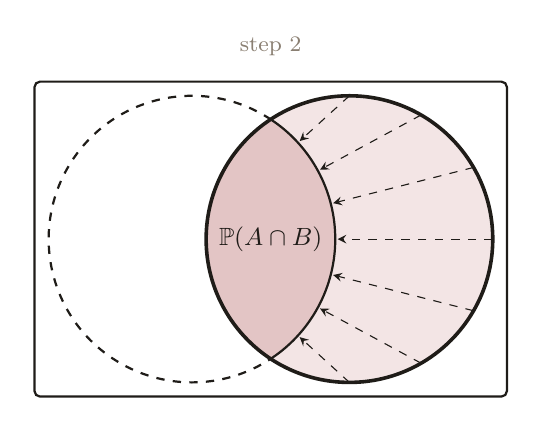
\begin{tikzpicture}[
  x=1cm,
  y=1cm,
  every node/.style={font=\normalsize},
  >=stealth
]
  \def\circleA{(0,0) circle (1.82)}
  \def\circleB{(2,0) circle (1.82)}
  \begin{scope}
    \path[fill=journalaccent, fill opacity=0.12] \circleB;
  \end{scope}
  \begin{scope}
    \clip \circleA;
    \path[fill=journalaccent, fill opacity=0.18] \circleB;
  \end{scope}
  \draw[journalink, line width=0.8pt, rounded corners=2pt] (-2,-2) rectangle (4,2);
  \draw[journalink, line width=1.3pt] \circleB;
  \draw[journalink, line width=0.8pt] ([shift=(-56.5:1.82)]0,0) arc (-56.5:56.5:1.82);
  \draw[journalink, line width=0.8pt, dashed] ([shift=(56.5:1.82)]0,0) arc (56.5:303.5:1.82);
  \node[journalink] at (1,0) {\small $\mathbb{P}(A\cap B)$};
  \node[journalmuted] at (1,2.45) {\footnotesize step 2};

  \draw[journalink, dashed, ->] (2.9100000,1.5761662) -- (1.6267097,0.8810876);
  \draw[journalink, dashed, ->] (2.000000,1.820000) -- (1.368270,1.245126);
  \draw[journalink, dashed, ->] (3.5761662,0.9100000) -- (1.7928653,0.4562169);
  \draw[journalink, dashed, ->] (3.82,0.00) -- (1.85,0.00);
  \draw[journalink, dashed, ->] (2.9100000,-1.5761662) -- (1.6267097,-0.8810876);
  \draw[journalink, dashed, ->] (2.000000,-1.820000) -- (1.368270,-1.245126);
  \draw[journalink, dashed, ->] (3.5761662,-0.9100000) -- (1.7928653,-0.4562169);
\end{tikzpicture}
\end{document}
